% phil379-print.tex
%
% driver file phil379-screen.tex to produce text on Crown Quarto
% size but all b/w for printing, and no cover

% We use the memoir class for maximal flexibility of layout, but any
% class will do

\documentclass[11pt,openany]{memoir}

\RequirePackage{amsthm}
\RequirePackage{xcolor}
\RequirePackage[usetwoside=false]{mdframed}
\RequirePackage[full]{textcomp}

% let's set the whole thing in Baskervald X, with Universalis ADF
% Standard for sans-serif, and spread the lines a bit to make the text
% more readable

\usepackage[sfdefault]{universalis}
\usepackage[osf]{Baskervaldx} % oldstyle figures
\usepackage[bigdelims,baskervaldx]{newtxmath} 
\usepackage[cal=boondoxo]{mathalfa}

% Make sure we have a copyright symbol

\def\copyright{\textcircled{C}}

\def\oljobname{phil379}

% next line needed for Adobe Acrobat to open the PDF.  may have
% somethign to do with transparency in the PNG graphics files?

\pdfminorversion=4

% set stock & paper size to Lulu's Crown Quarto dimensions

\setstocksize{24.589cm}{18.91cm}

\settrimmedsize{\stockheight}{\stockwidth}{*}
\settrims{0pt}{0pt}

% let's calculate the line length for 65 characters in \normalfont

\setlxvchars

% set the size of the type block to golden ratio calculated width

\settypeblocksize{*}{1.05\lxvchars}{1.62}

% set spine and and edge margin

\setlrmargins{*}{*}{1.3}
\setulmargins{80pt}{*}{*}
\setheaderspaces{*}{*}{1}

\checkandfixthelayout

% Chapter style

\makeatletter

\colorlet{leadbeater}{black}
\colorlet{dkleadbeater}{black}
\colorlet{ltleadbeater}{black!5}
\newlength{\barlength}
\makechapterstyle{leadbeater}{%
  \setlength{\afterchapskip}{40pt}
  \setlength{\beforechapskip}{50pt}
    \setlength{\midchapskip}{10pt}
  \renewcommand*{\afterchapternum}{\par\nobreak\vskip 0pt}
  \renewcommand*{\chapnamefont}{\fontsize{14pt}{0pt}\selectfont\bfseries\sffamily}
  \renewcommand*{\chapnumfont}{\fontsize{14pt}{0pt}\selectfont\bfseries\sffamily}
  \renewcommand*{\chaptitlefont}{\normalfont\fontsize{48pt}{48pt}\selectfont\bfseries\itshape\color{leadbeater}}
  \renewcommand*{\printchaptername}{%
    \chapnamefont\MakeUppercase{\@chapapp}}
  \renewcommand*{\printchaptertitle}[1]{%
    \chaptitlefont ##1\\[-\baselineskip]%
    \hspace*{-20pt}%
    \smash{\color{leadbeater}\rule{7pt}{250pt}}}
}

\renewcommand*{\partnamefont}{\fontsize{24pt}{0pt}\selectfont\bfseries\sffamily}
\renewcommand*{\partnumfont}{\fontsize{24pt}{0pt}\selectfont\bfseries\sffamily}
\renewcommand*{\parttitlefont}{\normalfont\fontsize{54pt}{54pt}\selectfont\bfseries\itshape\color{leadbeater}}
\renewcommand*{\printpartname}{%
  \partnamefont PART}

\makeatother

\chapterstyle{leadbeater}

\copypagestyle{leadbeater}{headings}

\makeevenhead{leadbeater}{\color{leadbeater}\sffamily\bfseries\thepage}{}
             {\small\sffamily\color{leadbeater}\leftmark}
\makeoddhead{leadbeater}{\small\sffamily\color{leadbeater}\rightmark}{}
            {\color{leadbeater}\sffamily\bfseries\thepage}

\usepackage[font={small,it}]{caption}


% \olpath has to point to the location of the OLP main
% directory/folder.  We're compiling from subdirectory
% courses/phil379/, so the main directory is two
% levels up.

\newcommand{\olpath}{../../}

% load all the Open Logic definitions. This will also load the
% local definitions in open-logic-sample-config.sty

\input{\olpath/sty/open-logic.sty}

% we want all the problems deferred to the very end

\input{\olpath/sty/open-logic-defer.sty}

% use high-res versions of photos

\tagfalse{olphotos-lowres}

% all links plain black for printing

\hypersetup{hidelinks}

% end preamble           

\begin{document}

% load the text

% phil379.tex
%
% driver file phil379.tex to produce text

\frontmatter

% bastard title

\pagestyle{empty}

\vspace*{100pt}

\begin{raggedleft}
{\fontsize{24pt}{24pt}\selectfont\bfseries\sffamily%
  Sets, Logic, Computation}
\end{raggedleft}


\newpage

% editorial board

\vspace*{100pt}

{\bfseries\itshape The Open Logic Project}

\bigskip

\textbf{\color{leadbeater}Instigator}

\medskip

Richard Zach, \emph{University of Calgary}

\bigskip

\textbf{\color{leadbeater}Editorial Board}

\medskip

Aldo Antonelli,$^\dagger$ \emph{University of California, Davis}

Andrew Arana, \emph{Universit\'e Paris I Panth\'enon--Sorbonne}

Jeremy Avigad, \emph{Carnegie Mellon University}

Walter Dean, \emph{University of Warwick}

Gillian Russell, \emph{University of North Carolina}

Nicole Wyatt, \emph{University of Calgary}

Audrey Yap, \emph{University of Victoria}

\bigskip

\textbf{\color{leadbeater}Contributors}

\medskip

Samara Burns, \emph{University of Calgary}

Dana H\"agg, \emph{University of Calgary}

\newpage

% title

\vspace*{100pt}

\begin{raggedleft}

{\fontsize{24pt}{24pt}\selectfont\bfseries\sffamily%
  Sets, Logic, Computation}

\smallskip

{\fontsize{18pt}{18pt}\selectfont\bfseries\itshape An Open Logic Text}

\vspace{100pt}

\fontsize{14pt}{14pt}\selectfont Remixed by Richard Zach

\vfill

\textsc{winter 2016}

\end{raggedleft}


\newpage

% copyright

\noindent
The Open Logic Project would like to acknowledge the generous support
of the Faculty of Arts of the University of Calgary and the Alberta
OER Initiative.

\bigskip

\noindent
\includegraphics[width=4cm]{aboer-color}

\bigskip

\noindent
\includegraphics[width=5cm]{ucarts-color}

\vfill

\noindent Illustrations by \href{http://mattleadbeater.com}{Matthew
  Leadbeater}, used under a
\href{http://creativecommons.org/licenses/by-nc/4.0/}{Creative Commons
  Attribution-NonCommercial 4.0 International License}.

\vfill

\noindent Typeset in Baskervald X and Universalis ADF Standard by
\LaTeX.

\vfill

% oluselicense generates a license mark that a) licenses the result
% under a CC-BY licence and b) acknowledges the original source (the
% OLP).  Acknowledgment of the source is a requirement under the
% conditions of the CC-BY license used by the OLP, but you are not
% required to license the product itself under CC-BY.

\renewcommand{\ollicensefont}{\fontsize{9pt}{12pt}\selectfont}

\noindent
\oluselicense
% Title of this version of the OLT with link to source
{\href{https://github.com/rzach/phil379}{\textit{Sets, Logic,
Computation}}}
% Author of this version
{\href{http://richardzach.org/}{Richard Zach}}

\newpage
\pagestyle{leadbeater}
\currentpdfbookmark{Table of Contents}{name}
\tableofcontents*

\cleartoverso
\thispagestyle{empty}
\ \vfill
\noindent\hskip-1cm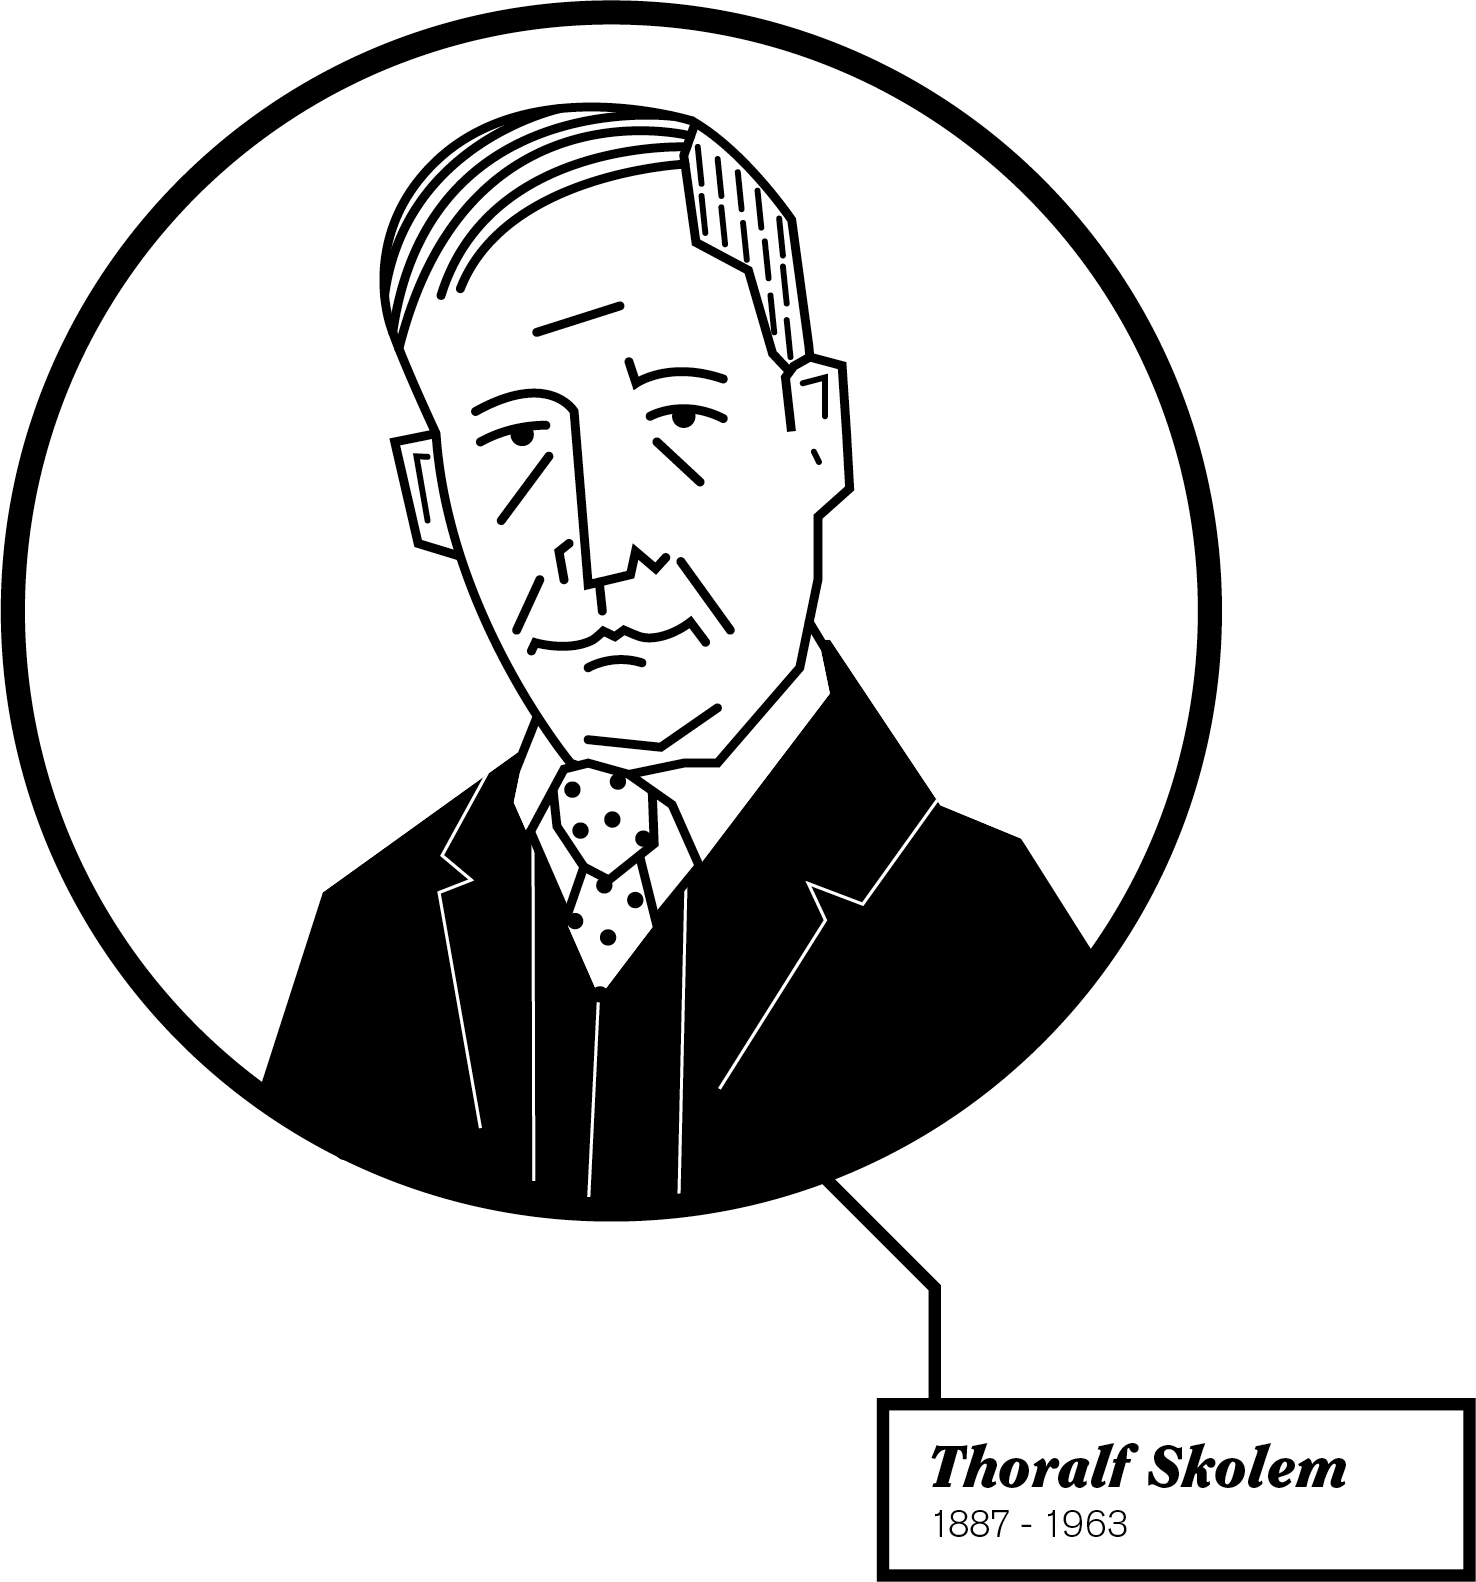
\includegraphics{illustrations/SkolemChapter}
\vfill

\chapter{Preface}

This book is an introduction to meta-logic, aimed especially at
students of computer science and philosophy.  ``Meta-logic'' is
so-called because it is the discipline that studies logic itself.
Logic proper is concerned with canons of valid inference, and its
symbolic or formal version presents these canons using formal
languages, such as those of propositional and predicate, a.k.a.,
first-order logic.  Meta-logic investigates the properties of these
language, and of the canons of correct inference that use them.  It
studies topics such as how to give precise meaning to the expressions
of these formal languages, how to justify the canons of valid
inference, what the properties of various proof systems are, including
their computational properties.  These questions are important and
interesting in their own right, because the languages and proof
systems investigated are applied in many different areas---in
mathematics, philosophy, computer science, and linguistics,
especially---but they also serve as examples of how to study formal
systems in general.  The logical languages we study here are not the
only ones people are interested in.  For instance, linguists and
philosophers are interested in languages that are much more
complicated than those of propositional and first-order logic, and
computer scientists are interested in other \emph{kinds} of languages
altogether, such as programming languages.  And the methods we discuss
here---how to give semantics for formal languages, how to prove
results about formal languages, how to investigate the properties of
formal languages---are applicable in those cases as well.

Like any discipline, meta-logic both has a set of results or facts,
and a store of methods and techniques, and this text covers both.
Some students won't need to know some of the results we discuss
outside of this course, but they will need and use the methods we use
to establish them.  The L\"owenheim-Skolem theorem, say, does not
often make an appearance in computer science, but the methods we use
to prove it do.  On the other hand, many of the results we discuss do
have relevance for certain debates, say, in the philosophy of science
and in metaphysics. Philosophy students may not need to be able to
prove these results outside this course, but they do need to
understand what the results are---and you really only
\emph{understand} these results if you have thought through the
definitions and proofs needed to establish them.  These are, in part,
the reasons for why the results and the methods covered in this text
are recommended study---in some cases even required---for students of
computer science and philosophy.

The material is divided into three parts.  Part~1 concerns
itself with the theory of sets.  Logic and meta-logic is historically
connected very closely to what's called the ``foundations of
mathematics.''  Mathematical foundations deal with how ultimately
mathematical objects such as integers, rational, and real numbers,
functions, spaces, etc., should be understood.  Set theory provides
one answer (there are others), and so set theory and logic have long
been studied side-by-side.  Sets, relations, and functions are also
ubiquitous in any sort of formal investigation, not just in
mathematics but also in computer science and in some of the more
technical corners of philosophy.  Certainly for the purposes of
formulating and proving results about the semantics and proof theory
of logic and the foundation of computability it is essential to have a
language in which to do this.  For instance, we will talk about sets
of expressions, relations of consequence and provability,
interpretations of predicate symbols (which turn out to be relations),
computable functions, and various relations between and constructions
using these.  It will be good to have shorthand symbols for
these, and think through the general properties of sets, relations,
and functions in order to do that.  If you are not used to thinking
mathematically and to formulating mathematical proofs, then think of
the first part on set theory as a training ground: all the basic
definitions will be given, and we'll give increasingly complicated
proofs using them.  Note that understanding these proofs---and being
able to find and formulate them yourself---is perhaps more important
than understanding the results, and especially in the first part, and
especially if you are new to mathematical thinking, it is important
that you think through the examples and do the problems in \cref{problems}.

In the first part we will establish one important result, however.
This result---Cantor's theorem---relies on one of the most striking
examples of conceptual analysis to be found anywhere in the sciences,
namely, Cantor's analysis of infinity.  Infinity has puzzled
mathematicians and philosophers alike for centuries. No-one knew how
to properly think about it. Many people even thought it was a mistake
to think about it at all, that the notion of an infinite object or
infinite collection itself was incoherent.  Cantor made infinity into
a subject we can coherently work with, and developed an entire theory
of infinite collections---and infinite numbers with which we can
measure the sizes of infinite collections---and showed that there are
different levels of infinity.  This theory of ``transfinite'' numbers
is beautiful and intricate, and we won't get very far into it; but we
will be able to show that there are different levels of infinity,
specifically, that there are ``countable'' and ``uncountable'' levels
of infinity.  This result has important applications, but it is
also really the kind of result that any self-respecting mathematician,
computer scientist, or philosopher should know.

In the second part we turn to first-order logic.  We will define the
language of first-order logic and its semantics, i.e., what first-order
structures are and when a sentence of first-order logic is true in a
structure.  This will enable us to do two important things: (1) We can
define, with mathematical precision, when a sentence is a logical
consequence of another.  (2) We can also consider how the relations
that make up a first-order structure are
described---characterized---by the sentences that are true in them.
This in particular leads us to a discussion of the axiomatic method,
in which sentences of first-order languages are used to characterize
certain kinds of structures.  Proof theory will occupy us next, and we
will consider the original version of natural deduction as defined in
the 1930s by Gerhard Gentzen.  The semantic notion of consequence and
the syntactic notion of provability give us two completely different
ways to make precise the idea that a sentence may follow from some
others. The soundness and completeness theorems link these two
characterization. In particular, we will prove G\"odel's completeness
theorem, which states that whenever a sentence is a semantic
consequence of some others, there is also a deduction of said sentence
from these others.  An equivalent formulation is: if a collection of
sentences is consistent---in the sense that nothing contradictory can
be proved from them---then there is a structure that makes all of them
true.

The second formulation of the completeness theorem is perhaps the more
surprising. Around the time G\"odel proved this result (in 1929), the
German mathematician David Hilbert famously held the view that
consistency (i.e., freedom from contradiction) is all that mathematical
existence requires.  In other words, whenever a mathematician can
coherently describe a structure or class of structures, then they
should be be entitled to believe in the existence of such structures.
At the time, many found this idea preposterous: just because you can
describe a structure without contradicting yourself, it surely does
not follow that such a structure actually exists.  But that is exactly
what G\"odel's completeness theorem says.  In addition to this
paradoxical---and certainly philosophically intriguing aspect---the
completeness theorem also has two important applications which allow
us to prove further results about the existence of structures which
make given sentences true.  These are the compactness and the
L\"owenheim-Skolem theorem.

In the third part, we connect logic with computability.  Again, there
is a historical connection: David Hilbert had posed as a fundamental
problem of logic to find a mechanical method which would decide, of a
given sentence of logic, whether it has a proof. Such a method exists,
of course, for propositional logic: one just has to check all truth
tables, and since there are only finitely many of them, the method
eventually yields a correct answer.  Such a straightforward method is
not possible for first-order logic, since the number of possible
structures is infinite (and structures themselves may be
infinite). Logicians were working on finding a more ingenious methods
for years.  Two logicians---Alonzo Church and Alan Turing---eventually
established that there is no such method.  In order to do this, it was
necessary to first provide a precise definition of what a
mechanical method is in general. If an effective method had been
proposed, anyone would have recognized it as an effective method. To
prove that no effective method exists, you have to define ``effective
method'' first and give an impossibility proof on the basis of that
definition.  This is what Turing did: he proposed the idea of a Turing
machine\footnote{Turing of course did not call it that himself.} as a
mathematical model of what a mechanical procedure can, in principle,
do.  This is another example of a \emph{conceptual analysis} of an
informal concept using mathematical machinery; and it is perhaps of
the same order of importance for computer science as Cantor's analysis
of infinity is for mathematics.  Our last major undertaking will be
the proof of two impossibility theorems: we will show that the
so-called ``halting problem'' cannot be solved by Turing machines, and
finally that Hilbert's ``decision problem'' (for logic) also cannot.

This text is mathematical, in the sense that we discuss mathematical
definitions and prove our results mathematically.  But it is not
mathematical in the sense that you need extensive mathematical
background knowledge.  Nothing in this text requires advanced
knowledge of algebra, trigonometry, or calculus.  We have made a
special effort to also not require any familiarity with the way
mathematics works: in fact, part of the point is to \emph{develop} the
kinds of reasoning and proof skills required to understand and prove
our results.  The organization of the text follows mathematical
convention, for one reason: these conventions have been developed
because clarity and precision are especially important, and so, e.g.,
it is critical to know when something is asserted as the conclusion of
an argument, is offered as a reason for something else, or is intended
to introduce new vocabulary. So we follow mathematical convention and
label passages as ``definitions'' if they are used to introduce new
terminology or symbols; and as ``theorems,'' ``propositions,''
``lemmas,'' or ``corollaries'' when we record a result or
finding.\footnote{The difference between the latter four is not
  terribly important, but roughly: A theorem is an important result. A
  proposition is a result worth recording, but perhaps not as
  important as a theorem. A lemma is a result we mainly record only
  because we want to break up a proof into smaller, easier to manage
  chunks.  A corollary is a result that follows easily from a theorem
  or proposition, such as an interesting special case.}  Other than
these conventions, we will only use the methods of logical proof as
they should be familiar from a first logic course, with one exception:
we will make extensive use of the method of \emph{induction} to prove
results.  A chapter of the appendix is devoted to this principle.



\cleartoverso 


\thispagestyle{empty}
\ \vfill
\noindent\hskip-1cm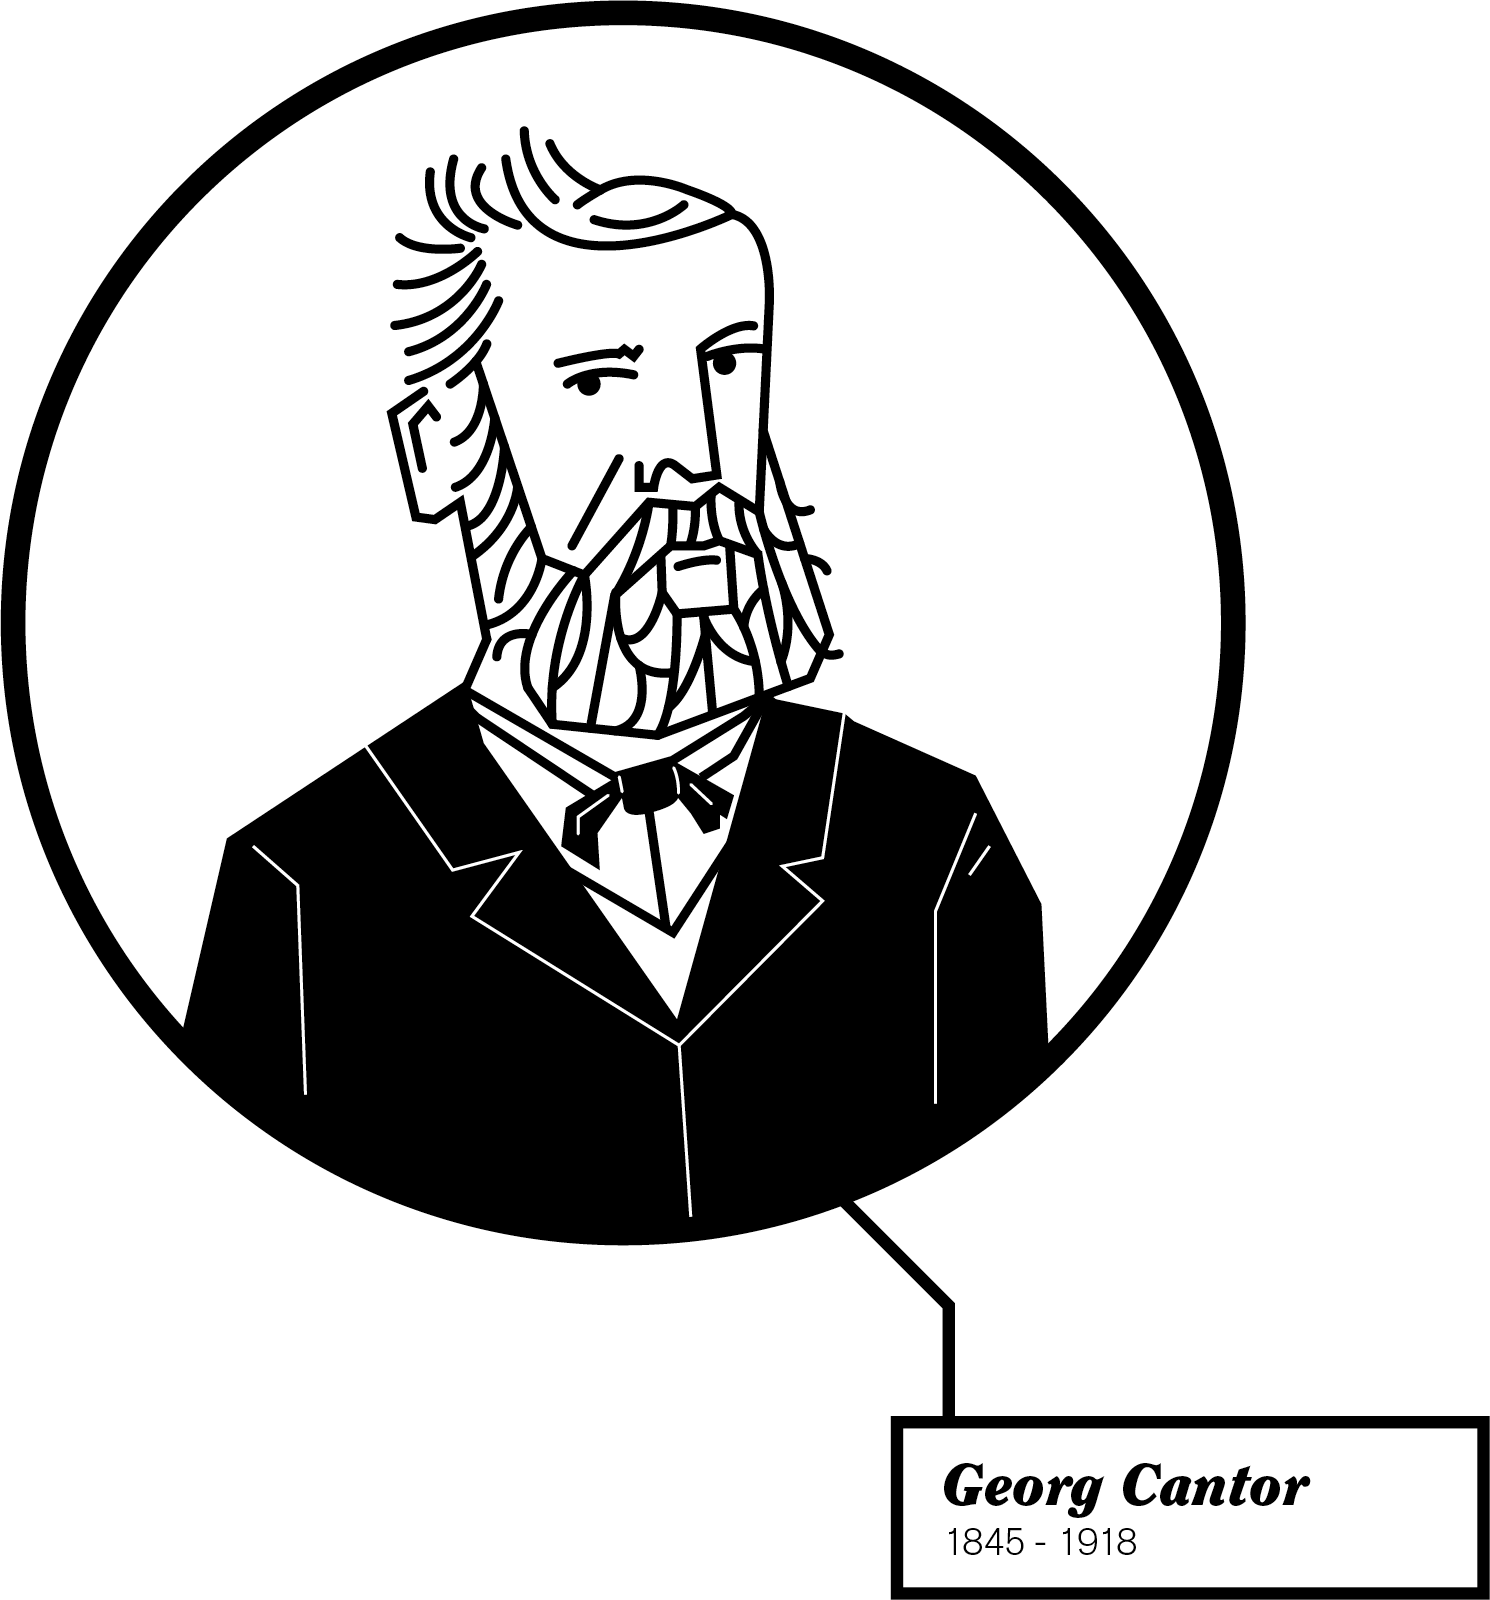
\includegraphics{illustrations/CantorChapter}
\vfill

\mainmatter

\pagestyle{leadbeater}

\olimport*[sets-functions-relations]{sets-functions-relations}

\cleartoverso
\ifodd\value{page}\stepcounter{page}\fi
\thispagestyle{empty}
\ \vfill
\noindent\hskip-1cm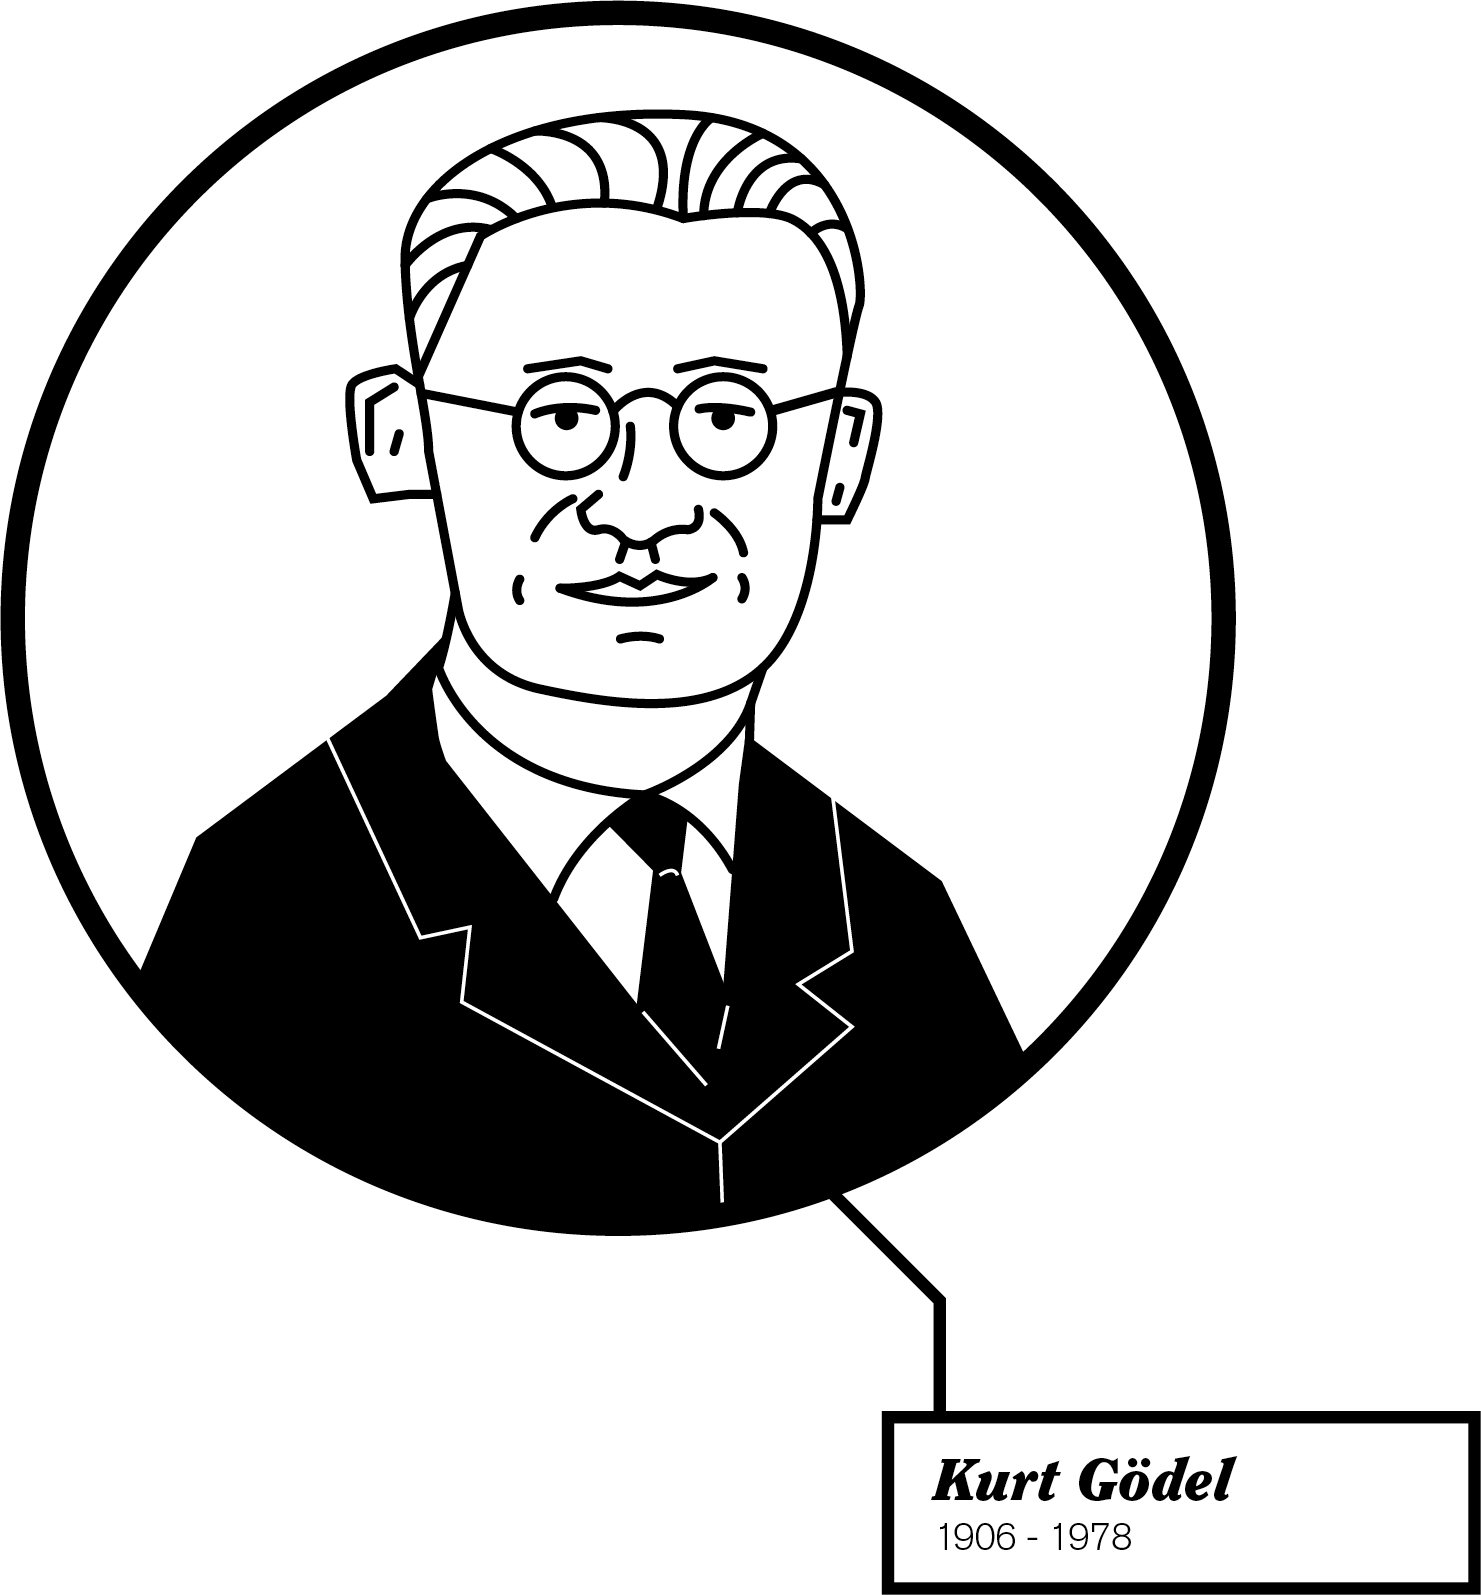
\includegraphics{illustrations/GodelChapter}
\vfill

\olimport*[first-order-logic]{first-order-logic}

\cleartoverso
\ifodd\value{page}\stepcounter{page}\fi
\thispagestyle{empty}
\ \vfill
\noindent\hskip-1cm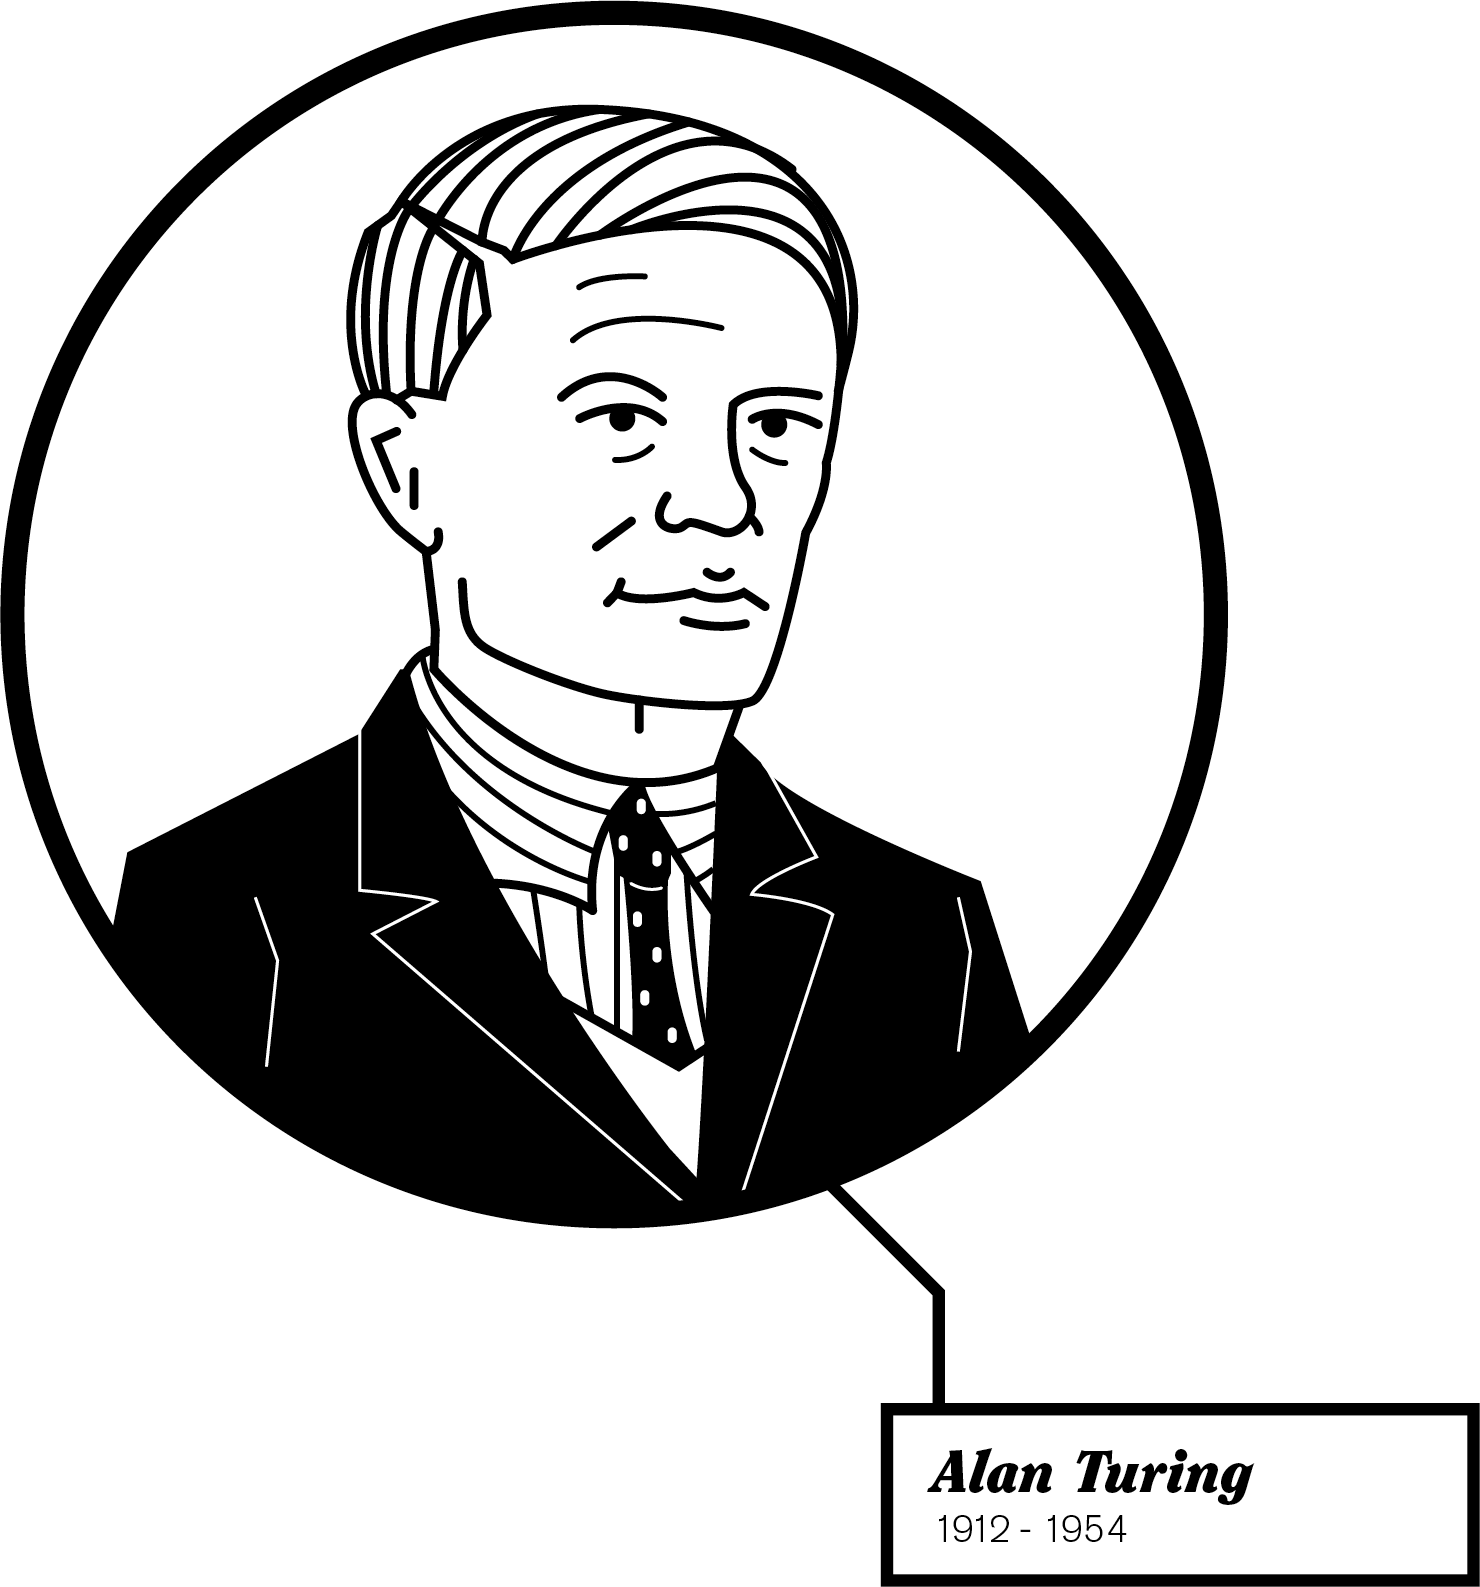
\includegraphics{illustrations/TuringChapter}
\vfill

\olimport*[turing-machines]{turing-machines}

\stopproblems

% now typeset all the problems as an appendix. If you want problems at
% the end of each chapter, delete this part and put
% \problemsperchapter in the preamble

\cleartoverso
\ifodd\value{page}\stepcounter{page}\fi
\thispagestyle{empty}
\ \vfill
\noindent\hskip-1cm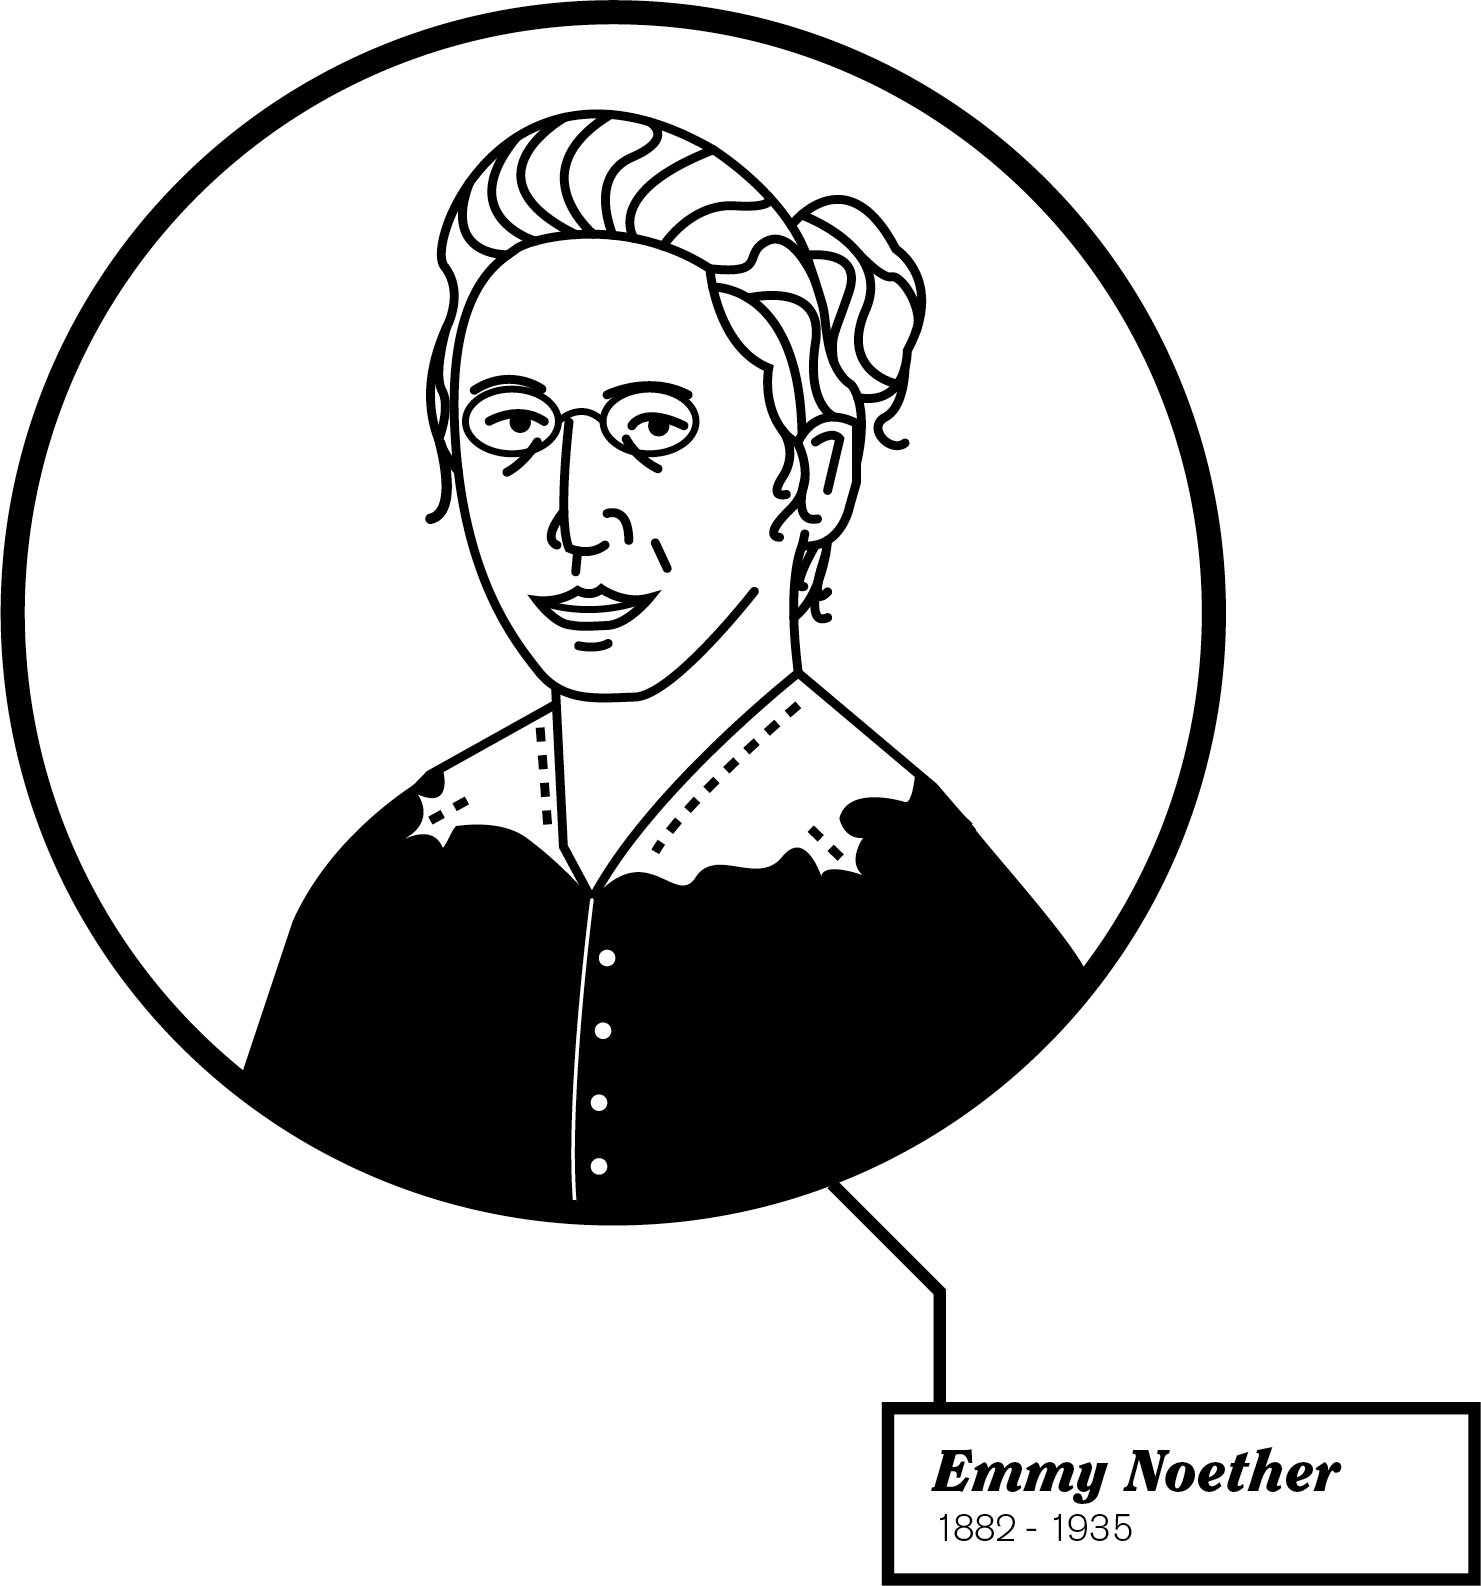
\includegraphics{illustrations/NoetherChapter}
\vfill

\appendix

\olimport{induction}
\def\captionnamefont{\sffamily\color{leadbeater}}
\def\captiontitlefont{\sffamily\color{leadbeater}}

\def\figurename{Fig.}
\setlength{\olphotowidth}{.45\textwidth}

\olimport*[history/biographies]{biographies}

\chapter{Problems}

\label{problems}

\printproblems

\backmatter

\photocredits

\bibliographystyle{\olpath/bib/natbib-oup}
\bibliography{\olpath/bib/open-logic.bib}

\olimport*{\olpath/content/open-logic-about}


\end{document}

